\cleardoublepage
\mbox{}


\chapter{Tecnología Openvino}
\label{ch:chapter3}


\section{Herramientas que lo componen}
Esta tecnología desarrollada por intel se centra principalmente en la optimización de modelos de redes neuronales convolucionales para potenciar su velocidad de inferencia mediante las distintas herramientas que lo componen.
Esta herramienta soporta distintos hardwares como FPGA, Intel movidius, procesamiento por GPU\@ y también distintos sistemas operativos como Mac Os, Linux o Windows.
Las características principales de esta aplicación se resumen en dos puntos :
\begin{itemize}
    \item \textbf{Optimizador de modelos de deep learning}: Aplicación CLI la cual usa como base modelos de frameworks populares como Caffe, TensorFlow, MXNet, Kaldi y ONNX para convertirlos a un modelo optimizado de Openvino.
    \item \textbf{Interfaz de inferencia de modelos de deep learning}: API de alto rendimiento multi plataforma para realizar la inferencia de manera rápida.
\end{itemize}

Es una aplicación multi plataforma que facilita la transición entre entre los entornos de entrenamiento y producción de nuestro modelo.
El cometido principal de esta aplicación es recoger el binario de un modelo previamente entrenado para poder optimizar cada capa de la topología de nuestra red neuronal y
poder transformarla finalmente en un formato válido para la interfaz de inferencia de Openvino, que será la que realice las predicciones en el entorno productivo.
Este nuevo formato puede ser leído de manera unificada por cualquier hardware que esté realizando la inferencia con la API de Openvino, por lo que el mismo procedimiento de inferencia de nuestro modelo
puede servir en cualquier plataforma.

\begin{figure}
    \centering
    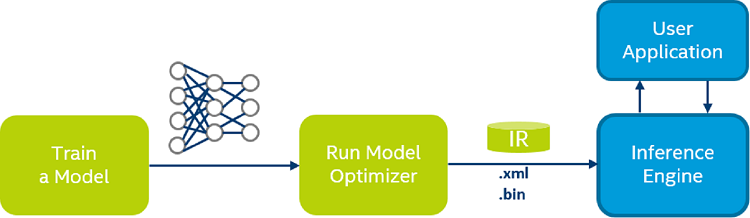
\includegraphics[width=0.8\textwidth]{images/openvino/model_optimizer.png}
    \caption{Arquitectura de optimización de modelos con Openvino}
    \label{fig:Arquitectura de optimización de modelos con Openvino}
\end{figure}

API de alto rendimiento para mejorar la inferencia


\section{Conversión del modelo a la plataforma OpenVINO}\label{sec:conversión-del-modelo-a-la-plataforma-openvino}
(Aquí comentas los pasos que sigues)


\section{Inferencias. Tensorflow vs OpenVINO}\label{sec:inferencias.-tensorflow-vs-openvino}
(Los resultados no habría que ponerlos en teoría aquí, sino llevarlos al apartado